\documentclass[12pt]{article}

\usepackage{titling}
\newcommand{\subtitle}[1]{%
	\posttitle{%
		\par\end{center}
	\begin{center}\large#1\end{center}
	\vskip0.5em}%
}
\usepackage{longtable}
\usepackage{amsfonts, amsmath, amssymb, bm} %Math fonts and symbols
\usepackage{dcolumn, multirow} % decimal-aligned columns, multi-row cells
\usepackage{graphicx} % graphics commands
\usepackage{subfig}
\usepackage{float}
\usepackage[margin=1in]{geometry} % sets page layout
\usepackage{setspace}% allows toggling of double/single-spacing
\usepackage{verbatim}% defines environment for un-evaluated code
\usepackage{rotating}% defines commands for rotating text and floats
\usepackage[sort]{natbib}% defines citation commands and environments.
\usepackage{url}
\usepackage{caption}
\usepackage{endnotes}
\usepackage{psfrag}
\usepackage{epstopdf}
\usepackage{epsfig}
\usepackage[pdftex,
            pdfauthor={Tom Hanna},
            pdftitle={The Title},
            pdfsubject={The Subject},
            pdfkeywords={Some Keywords},
            pdfcreator={TeXstudio}]{hyperref}
\usepackage{fancyhdr, amsfonts, amsmath, amssymb, graphicx, color, fullpage}
\pagestyle{fancy}
\usepackage{fourier}
\usepackage[lf]{venturis}
\usepackage[T1]{fontenc}
\DeclareMathOperator*{\argmax}{arg\,max}

\usepackage{outlines}
\usepackage{enumitem}[shortlabels]
\setlist[enumerate,1]{label=\Roman*)}
\setlist[enumerate,2]{label=\Alph*)}
\setlist[enumerate,3]{label=\roman*)}
\setlist[enumerate,4]{label=\alph*)}


\setlength\parindent{0pt}
\setlength{\headsep}{0.2in}

\usepackage{tikz}
\usetikzlibrary{trees}

\usetikzlibrary{shapes,decorations,arrows,calc,arrows.meta,fit,positioning}
\tikzset{
    -Latex,auto,node distance =1 cm and 1 cm,semithick,
    state/.style ={ellipse, draw, minimum width = 0.7 cm},
    point/.style = {circle, draw, inner sep=0.04cm,fill,node contents={}},
    bidirected/.style={Latex-Latex,dashed},
    el/.style = {inner sep=2pt, align=left, sloped}
}


\usepackage[sectionbib]{chapterbib}

\title{Sample Lab Presentation: Lab 9}


\author{Tom Hanna \\ University of Houston \\  Department of Political Science \\ tlhanna@uh.edu}




\begin{document}
\clearpage\maketitle
\thispagestyle{empty}
\setcounter{page}{1}





	\lhead{Tom Hanna}

	\chead{Lab 9 Sample}

	\rhead{POLS6481}



	{\textcolor{white}.}











\newpage

\doublespacing

	{\textcolor{white}.}



\section*{Raw code}

\begin{verbatim}
> library(here)
here() starts at C:/Users/tomha/Documents/3 - R Studio Projects/Teaching/POLS6481-Spring2021-UH-lab
> library(foreign)
> library(tseries) #For lagging
Registered S3 method overwritten by 'quantmod':
  method            from
  as.zoo.data.frame zoo 

    ‘tseries’ version: 0.10-48

    ‘tseries’ is a package for time series analysis and computational finance.

    See ‘library(help="tseries")’ for details.

> library(lmtest) #For test for joint significance
Loading required package: zoo

Attaching package: ‘zoo’

The following objects are masked from ‘package:base’:

    as.Date, as.Date.numeric

> library(plm) #For plm command  --- if needed install.packages("plm")
> library(pglm)
Loading required package: maxLik
Loading required package: miscTools

Please cite the 'maxLik' package as:
Henningsen, Arne and Toomet, Ott (2011). maxLik: A package for maximum 
likelihood estimation in R. Computational Statistics 26(3), 443-458. 
DOI 10.1007/s00180-010-0217-1.

If you have questions, suggestions, or comments regarding the
 'maxLik' package, please use a forum or 'tracker' at maxLik's R-Forge site:
https://r-forge.r-project.org/projects/maxlik/
> #This is using data on non-democratic nations involvement in Militarized
> Interstate Disputes
> #(MIDS), the data is from the Correlates of War dataset. Additionally, 
> #there are variables from the Varieties of Democracy (VDEM) project and 
> from Jeff Colgan's
> #Revolutionary Leader's database. This is unbalanced panel data, so
> #I won't be using the PLM package. 
> library(readr)
> NDC <- read_csv(here("data","nondemocraciesconflict.csv"))

-- Column specification -----------------------------------------------------------------------------
cols(
  .default = col_double(),
  country_name = col_character(),
  v2lpname = col_logical(),
  v2reginfo = col_character(),
  leader = col_character(),
  stabb = col_character()
)
i Use `spec()` for the full column specifications.

Warning messages:
1: Missing column names filled in: 'X1' [1] 
2: Duplicated column names deduplicated: 'X1' => 'X1_1' [149] 
> View(NDC)
> names(NDC) #I like to do this because it makes organizing and using variables easier
  [1] "X1"                         "COWcode"                    "year"                      
  [4] "country_name"               "v2x_polyarchy"              "v2x_libdem"                
  [7] "v2x_partipdem"              "v2x_delibdem"               "v2x_egaldem"               
 [10] "v2x_regime"                 "v2x_regime_amb"             "v2x_ex_military"           
 [13] "v2x_ex_confidence"          "v2x_ex_direlect"            "v2x_ex_hereditary"         
 [16] "v2x_ex_party"               "v2x_neopat"                 "v2xnp_client"              
 [19] "v2x_frassoc_thick"          "v2x_jucon"                  "v2xlg_legcon"              
 [22] "v2x_cspart"                 "v2lpname"                   "v2exhoshog"                
 [25] "v2exremhog"                 "v2exdjdshg"                 "v2exdfvthg"                
 [28] "v2reginfo"                  "v2regint"                   "v2regendtype"              
 [31] "v2regimpgroup"              "v2regsupgroupssize"         "v2lgoppart"                
 [34] "v2dlencmps"                 "v2juhcind"                  "v2juncind"                 
 [37] "v2juhccomp"                 "v2jucomp"                   "v2jureview"                
 [40] "v2stfisccap"                "v2svstterr"                 "v2mecenefi"                
 [43] "v2mecenefm"                 "v2exl_legitideol"           "v2exl_legitideolcr_0"      
 [46] "v2exl_legitideolcr_1"       "v2exl_legitideolcr_2"       "v2exl_legitideolcr_3"      
 [49] "v2exl_legitideolcr_4"       "v2xpe_exlsocgr"             "v2x_gencl"                 
 [52] "v2x_rule"                   "v2xcl_prpty"                "v2xcs_ccsi"                
 [55] "v2x_clpol"                  "v2x_clpriv"                 "v2clfmove"                 
 [58] "v2xcl_dmove"                "v2cldmovem"                 "v2cldmovew"                
 [61] "v2cldiscm"                  "v2cldiscw"                  "v2clslavem"                
 [64] "v2clslavef"                 "v2clstown"                  "v2clprptym"                
 [67] "v2clprptyw"                 "v2clacjstm"                 "v2clacjstw"                
 [70] "e_legparty"                 "e_autoc"                    "e_peaveduc"                
 [73] "e_migdppc"                  "e_migdppcln"                "e_cow_exports"             
 [76] "e_cow_imports"              "e_total_fuel_income_pc"     "e_total_oil_income_pc"     
 [79] "e_miurbani"                 "e_mipopula"                 "e_civil_war"               
 [82] "e_miinteco"                 "v2exrmhgnp_0"               "v2exrmhgnp_1"              
 [85] "v2exrmhgnp_2"               "v2exrmhgnp_3"               "v2exrmhgnp_4"              
 [88] "v2exrmhgnp_5"               "v2exrmhgnp_6"               "v2exrmhgnp_7"              
 [91] "v2exrmhgnp_8"               "v2exctlhg_0"                "v2exctlhg_1"               
 [94] "v2exctlhg_2"                "v2exctlhg_3"                "v2exctlhg_4"               
 [97] "v2exctlhg_5"                "v2exctlhg_6"                "v2exctlhg_7"               
[100] "v2exctlhg_8"                "v2regsupgroups_0"           "v2regsupgroups_1"          
[103] "v2regsupgroups_2"           "v2regsupgroups_3"           "v2regsupgroups_4"          
[106] "v2regsupgroups_5"           "v2regsupgroups_6"           "v2regsupgroups_7"          
[109] "v2regsupgroups_8"           "v2regsupgroups_9"           "v2regsupgroups_10"         
[112] "v2regsupgroups_11"          "v2regsupgroups_12"          "v2regsupgroups_13"         
[115] "v2exl_legitlead"            "ccode.x"                    "onsets"                    
[118] "revonsets"                  "sideaonsets"                "force_onsets"              
[121] "force_revonsets"            "force_sideaonsets"          "leader"                    
[124] "age0"                       "age"                        "usedforce"                 
[127] "irregulartransition"        "foundingleader"             "foreigninstall"            
[130] "radicalideology"            "democratizing"              "revolutionaryleader"       
[133] "chg_executivepower"         "chg_politicalideology"      "chg_propertyownership"     
[136] "chg_womenandethnicstatus"   "chg_religioningovernment"   "chg_revolutionarycommittee"
[139] "totalcategorieschanged"     "muslim"                     "durable"                   
[142] "cinc"                       "majorpower"                 "peaceyears"                
[145] "dem"                        "conflict.status"            "trade"                     
[148] "rule.inverse"               "X1_1"                       "dispnum"                   
[151] "stabb"                      "ccode.y"                    "stday"                     
[154] "stmon"                      "styear"                     "endday"                    
[157] "endmon"                     "endyear"                    "sidea"                     
[160] "revstate"                   "revtype1"                   "revtype2"                  
[163] "fatality"                   "fatalpre"                   "hiact"                     
[166] "hostlev"                    "orig"                       "version"                   
[169] "outcome"                    "settle"                     "recip"                     
[172] "numa"                       "numb"                       "legitideol"                
[175] "nationalist"                "socialist"                  "conservative"              
[178] "autonomist"                 "religious"                  "totalcat"                  
[181] "mideology"                  "mnationalist"               "msocialist"                
[184] "mconservative"              "mautonomist"                "mreligious"                
[187] "initiator"                  "revisionist"                "policyrevisionist"         
[190] "regimerevisionist"          "territorialrevisionist"     "otherrevisionist"          
[193] "nonterritorial"             "backdown"                   "hostile"                   
[196] "hostileorig"                "hostilepolicy"              "hostileregime"             
[199] "personofleader"             "coldwar"                    "transformativeideology"    
[202] "cinc2"                     
> ## The following produces an error because there are duplicates - some countries (COWcodes) 
> ## appear in multiple disputes in the same year. This is okay, because at this point I am 
> ## just demonstrating how to copy the console output to LaTeX.
> 
> panelNDC <- pdata.frame(NDC, c("COWcode","year"))
Warning message:
In pdata.frame(NDC, c("COWcode", "year")) :
  duplicate couples (id-time) in resulting pdata.frame
 to find out which, use, e.g., table(index(your_pdataframe), useNA = "ifany")
> pdim(panelNDC)
Error in pdim.default(index[[1L]], index[[2L]]) : 
  duplicate couples (id-time)
> 
\end{verbatim}

\pagebreak

\section*{Part 2: Plots}

\begin{itemize}
\item Plot of 1984, peace years versus transformative ideology.

\begin{figure}[H]
\centering
\caption[]{Data from 1984}
\label{fig:ti-vs-peaceyears-1984}
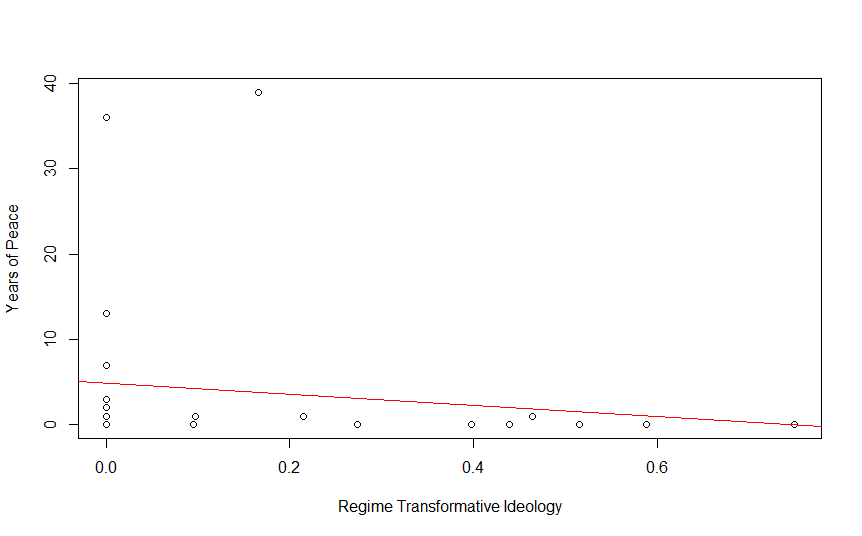
\includegraphics[width=0.9\linewidth]{ti-vs-peaceyears-1984}
\end{figure}



\item Plot of 1992, peace years versus transformative ideology.

\begin{figure}[H]
\centering
\caption[Data from 1992]{This is the plot of peace years versus transformative ideology for nondemocracies in 1992.}
\label{fig:ti-vs-oeaceyears-1992}
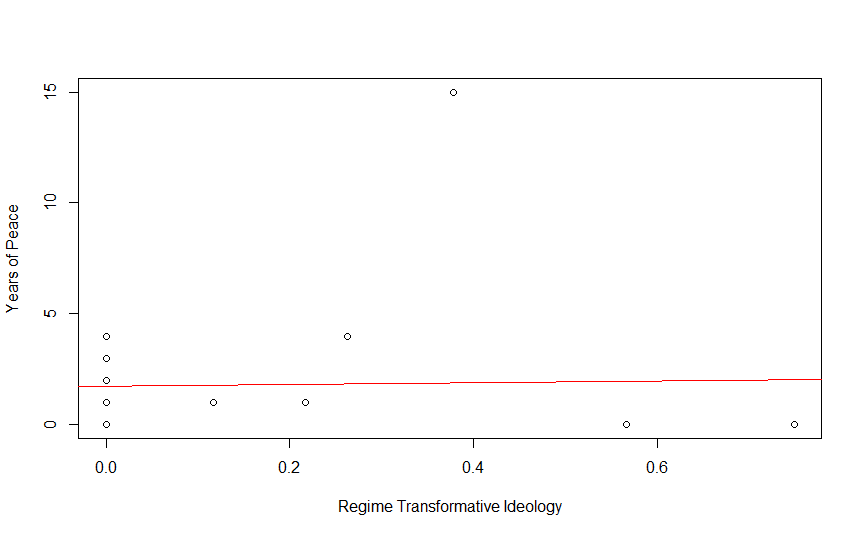
\includegraphics[width=0.9\linewidth]{ti-vs-oeaceyears-1992}
\end{figure}



\end{itemize}


\section*{Part 3: Results Tables}

\paragraph*{My results} show that XYZ (See Table 1, column Logit Model). As you can see in Table 1, the Logit Model was consistent with the Fixed Effects Logit Model.

% Table created by stargazer v.5.2.2 by Marek Hlavac, Harvard University. E-mail: hlavac at fas.harvard.edu
% Date and time: Tue, Apr 27, 2021 - 9:57:43 PM
\begin{table}[H] \centering 
  \caption{Transformative Ideology Effect on Nonterritorial Revisionist Demands} 
  \label{} 
\begin{tabular}{@{\extracolsep{5pt}}lcc} 
\\[-1.8ex]\hline 
\hline \\[-1.8ex] 
 & \multicolumn{2}{c}{\textit{Dependent variable:}} \\ 
\cline{2-3} 
\\[-1.8ex] & \multicolumn{2}{c}{Non-territorial Revisionist Demands} \\ 
\\[-1.8ex] & (Logit) & (Fixed Effects Logit Model)\\ 
\hline \\[-1.8ex] 
 Transformative Ideology & 1.056$^{***}$ & 0.778$^{**}$ \\ 
  & (0.205) & (0.375) \\ 
  & & \\ 
 Combined Index of & 0.030$^{***}$ & 0.044 \\ 
  National Capabilities & (0.011) & (0.036) \\ 
  & & \\ 
 Cold War & 0.157 & $-$0.026 \\ 
 (dummy variable) & (0.127) & (0.183) \\ 
  & & \\ 
 Peace Years & $-$0.023 & $-$0.026 \\ 
  & (0.015) & (0.020) \\ 
  & & \\ 
 Constant & $-$1.167$^{***}$ & $-$1.576$^{***}$ \\ 
  & (0.118) & (0.594) \\ 
  & & \\ 
\hline \\[-1.8ex] 
Observations & 1,768 & 1,768 \\ 
Log Likelihood & $-$1,059.119 & $-$861.691 \\ 
Akaike Inf. Crit. & 2,128.237 & 1,985.381 \\ 
\hline 
\hline \\[-1.8ex] 
\textit{Note: CFE ommitted for space}  & \multicolumn{2}{r}{$^{*}$p$<$0.1; $^{**}$p$<$0.05; $^{***}$p$<$0.01} \\ 
\end{tabular} 
\end{table} 


\newpage

\singlespacing

{\textcolor{white}.}

\bibliographystyle{apsr}

\bibliography{reference}





\end{document}

